\begin{task}{4, Chaotic dynamics}
In this task we will explore two dynamical systems with chaotic behaviour, the logistic map, and the Lorenz system. Both systems are implemented in the \verb|bifurcation.py| file and the plots are generated by \verb|visualization.py|. All the experiments for this task can be found inside the folder "task4" in the notebook \verb|experiments_task4.ipynb|.

Each of these systems have two functions inside \verb|bifurcation.py|. The function that computes the system in an atomic level, and the simulation function that runs the previous function for a given time. 

In addition, the logistic map has a \verb|warmup| parameter to discard a certain number of initial iterations when simulating the logistic map. This is done to allow the system to reach a steady state before collecting data for the plot. Then, the \verb|numtoplot| parameter is used to select the amount of final iterations to plot for each r value.

\paragraph{Logistic map}
The logistic map is defined as:
\[
x_{n+1} = rx_n(1-x_n), n \in \mathbb{N}
\]
We will study how the system behaves depending on the value of \(r\).
When we vary the value of \(r\) from 0 to 2, we can see how for \(0 \le r \le 1\) the system has a stable fixed point at \(x = 0\). For \(1 < r \le 3\) the system converges to the stable fixed point \(x_s = \frac{(r-1)}{r}\) \cite{strogatz2018nonlinear}. In Figure \ref{r02}  we observe this behaviour only for \(1 < r \le 2\). We can observe how a period-doubling bifurcation occurs, i.e. a slight change in a system's parameters causes a new periodic trajectory to emerge from an existing periodic trajectory.
\begin{figure}[H]
    \centering
    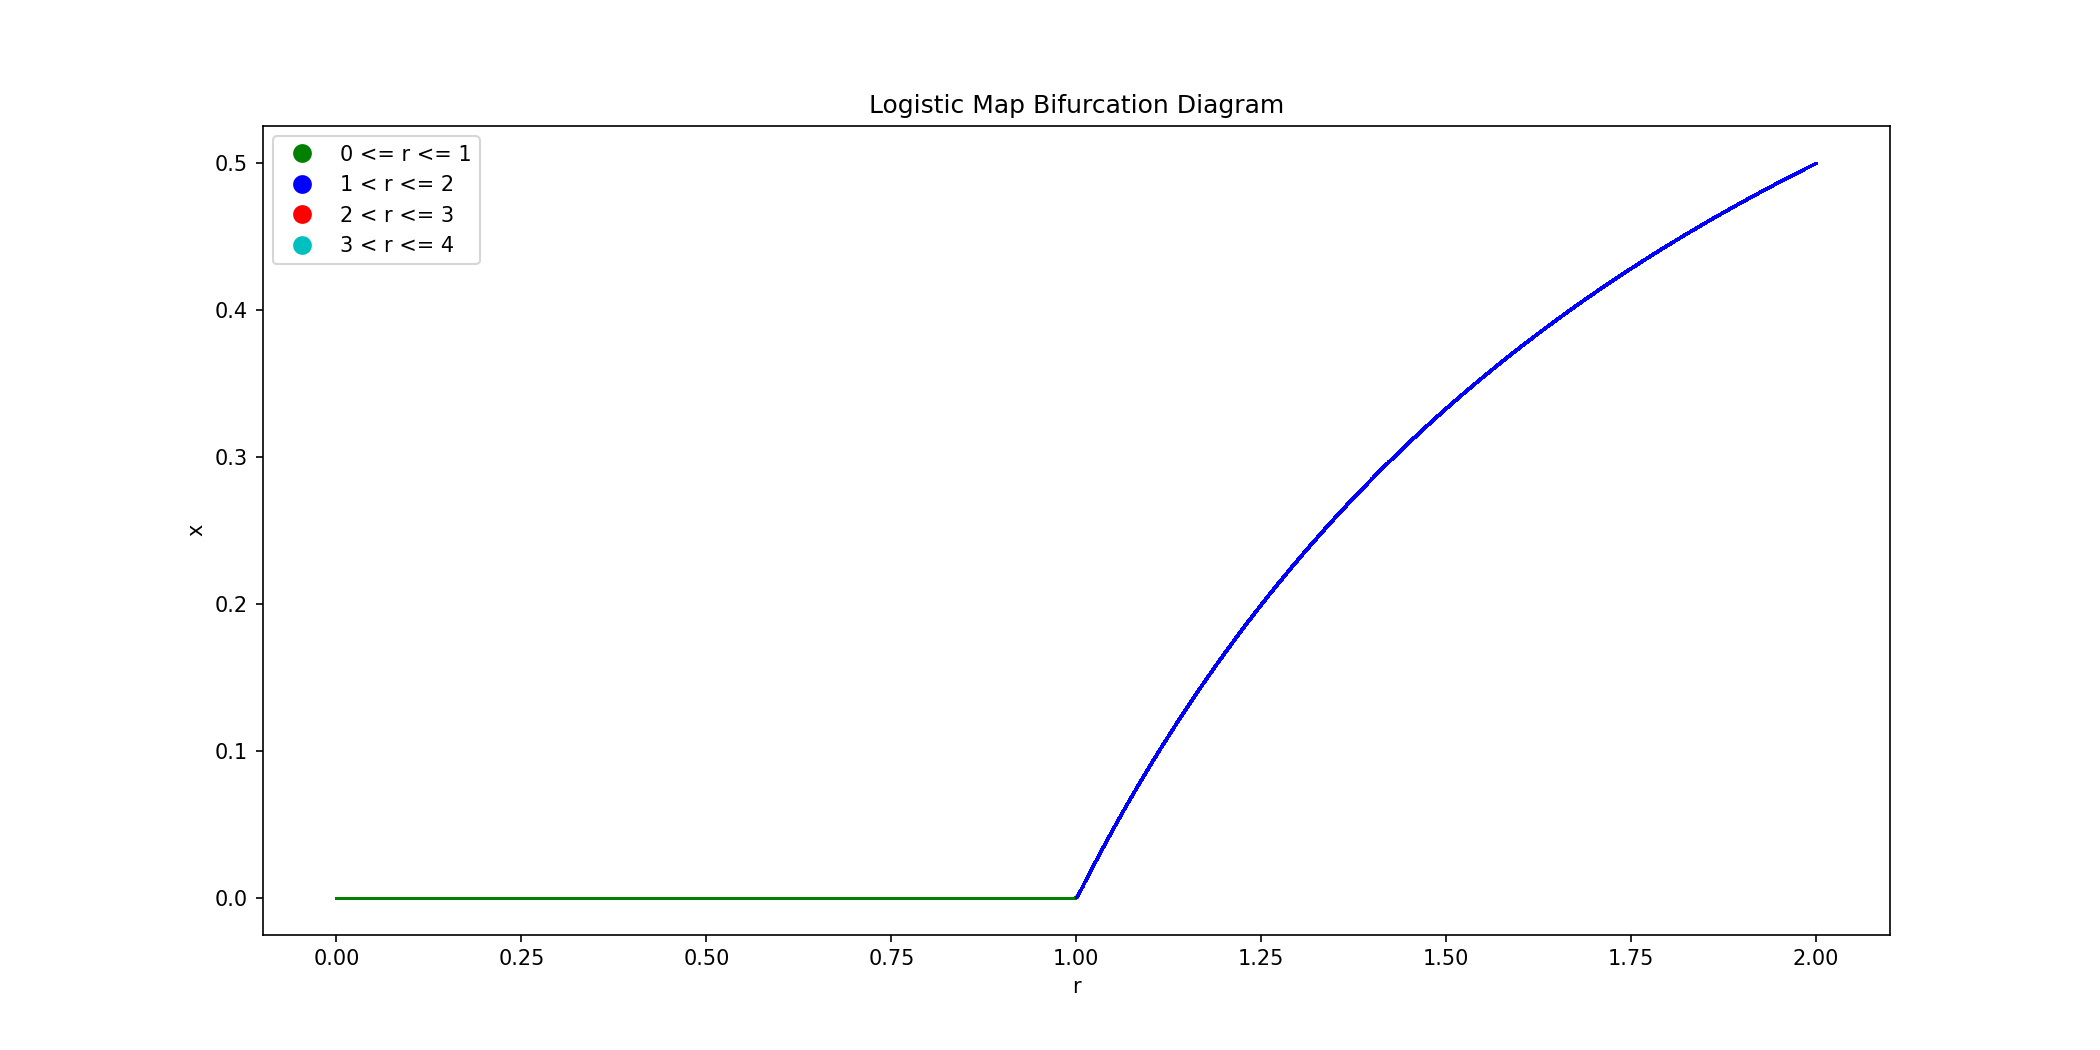
\includegraphics[width=0.75\textwidth]{images/logistic_map_0_2.png}
    \caption{Logistic map \(r \in [0,2]\)}
    \label{r02}
\end{figure}

On the other hand, when we vary the value of \(r\) from 2 to 4, we can observe a distinct behaviour. As \(r\) continues to increase, subsequent period-doubling bifurcations occur, leading to stable orbits. However, when \(r\) is approximately greater than 3.57 the system undergoes a transition to chaos. This is a sudden and qualitative change in behavior characterized by aperiodic, apparently random dynamics. The system shows extremely high sensitivity to initial conditions, and its long-term behavior becomes unpredictable \cite{gleick2008chaos}.

\begin{figure}[H]
    \centering
    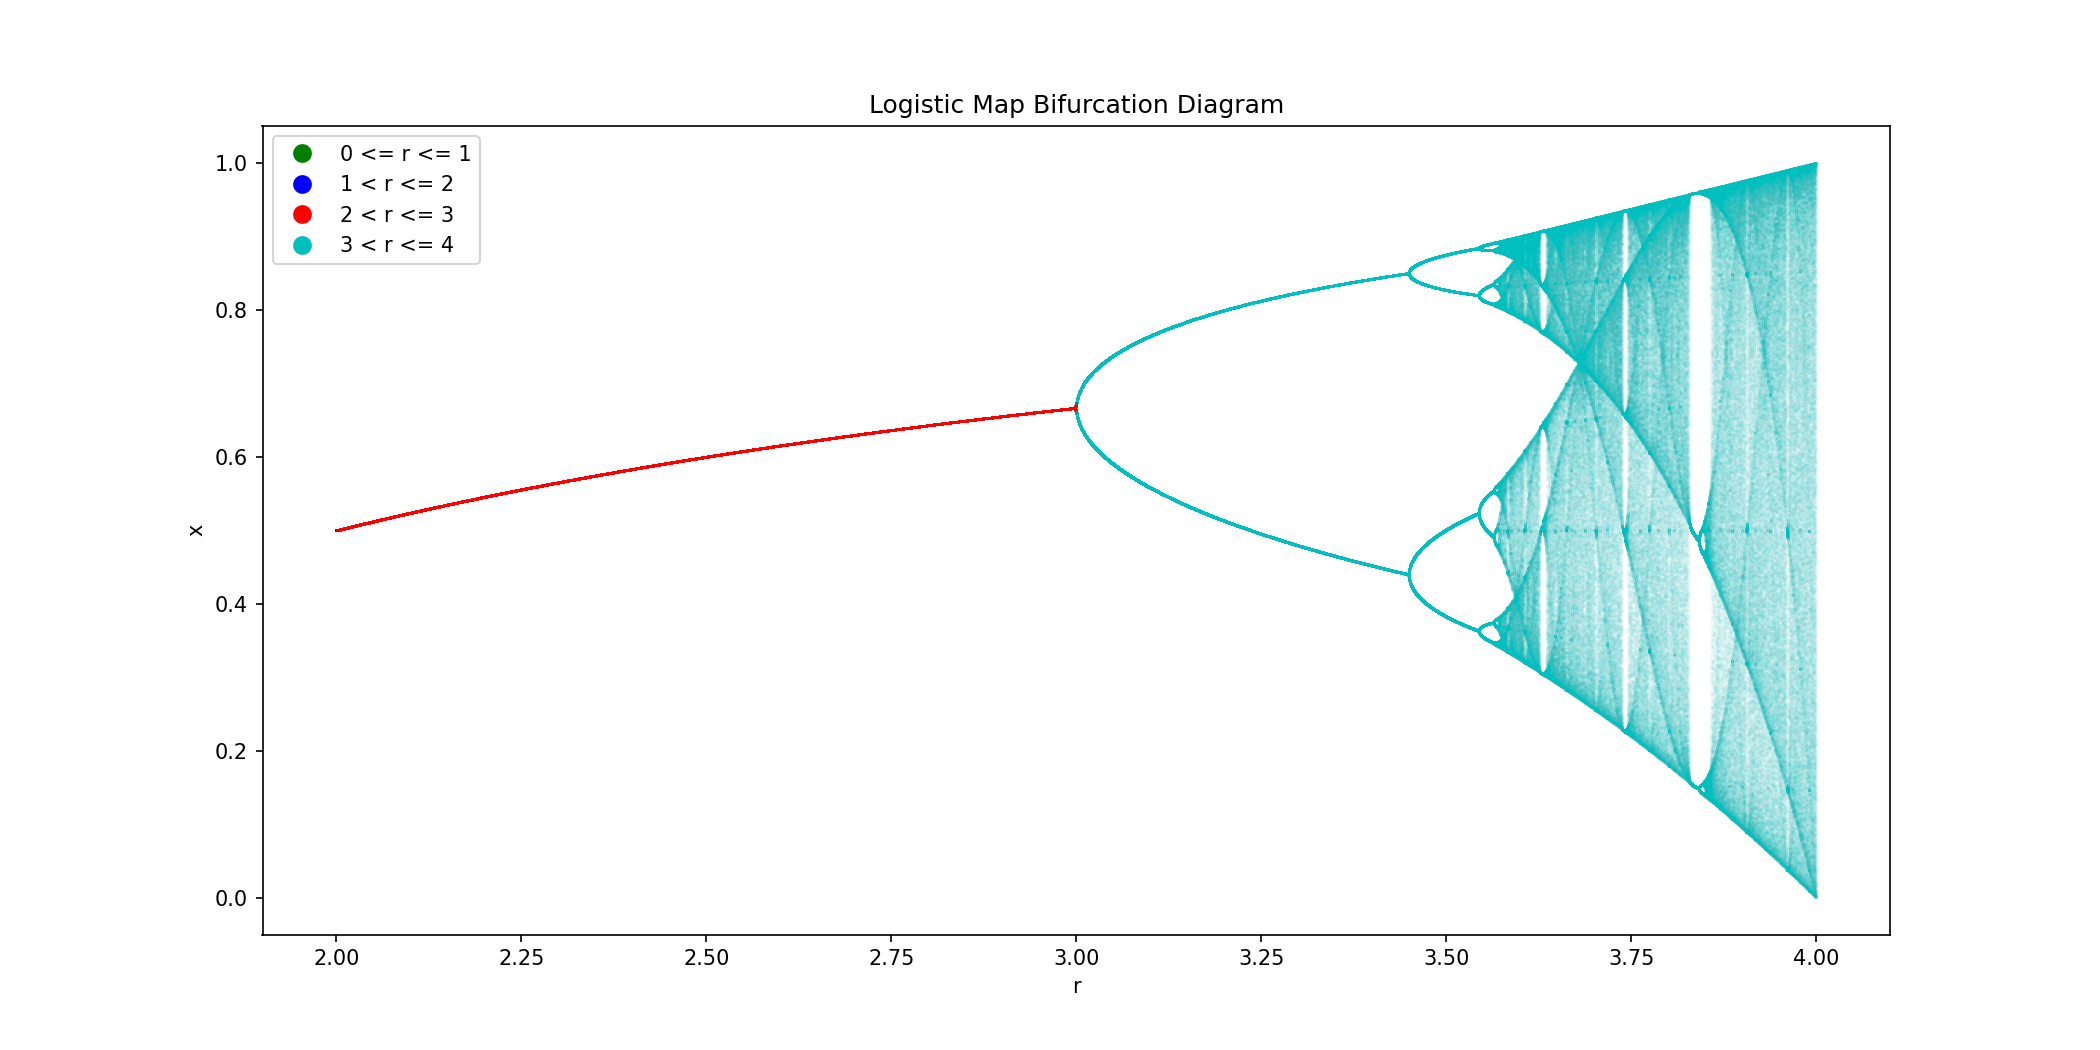
\includegraphics[width=0.75\textwidth]{images/logistic_map_2_4.png}
    \caption{Logistic map \(r \in [2,4]\)}
    \label{r24}
\end{figure}

Moreover, if we look closely Figure \ref{r34} we can observe what appear to be stable regions within the chaotic region, i.e. we can find again period-doubling bifurcations inside the big gaps left by the chaotic trajectory.

\begin{figure}[H]
    \centering
    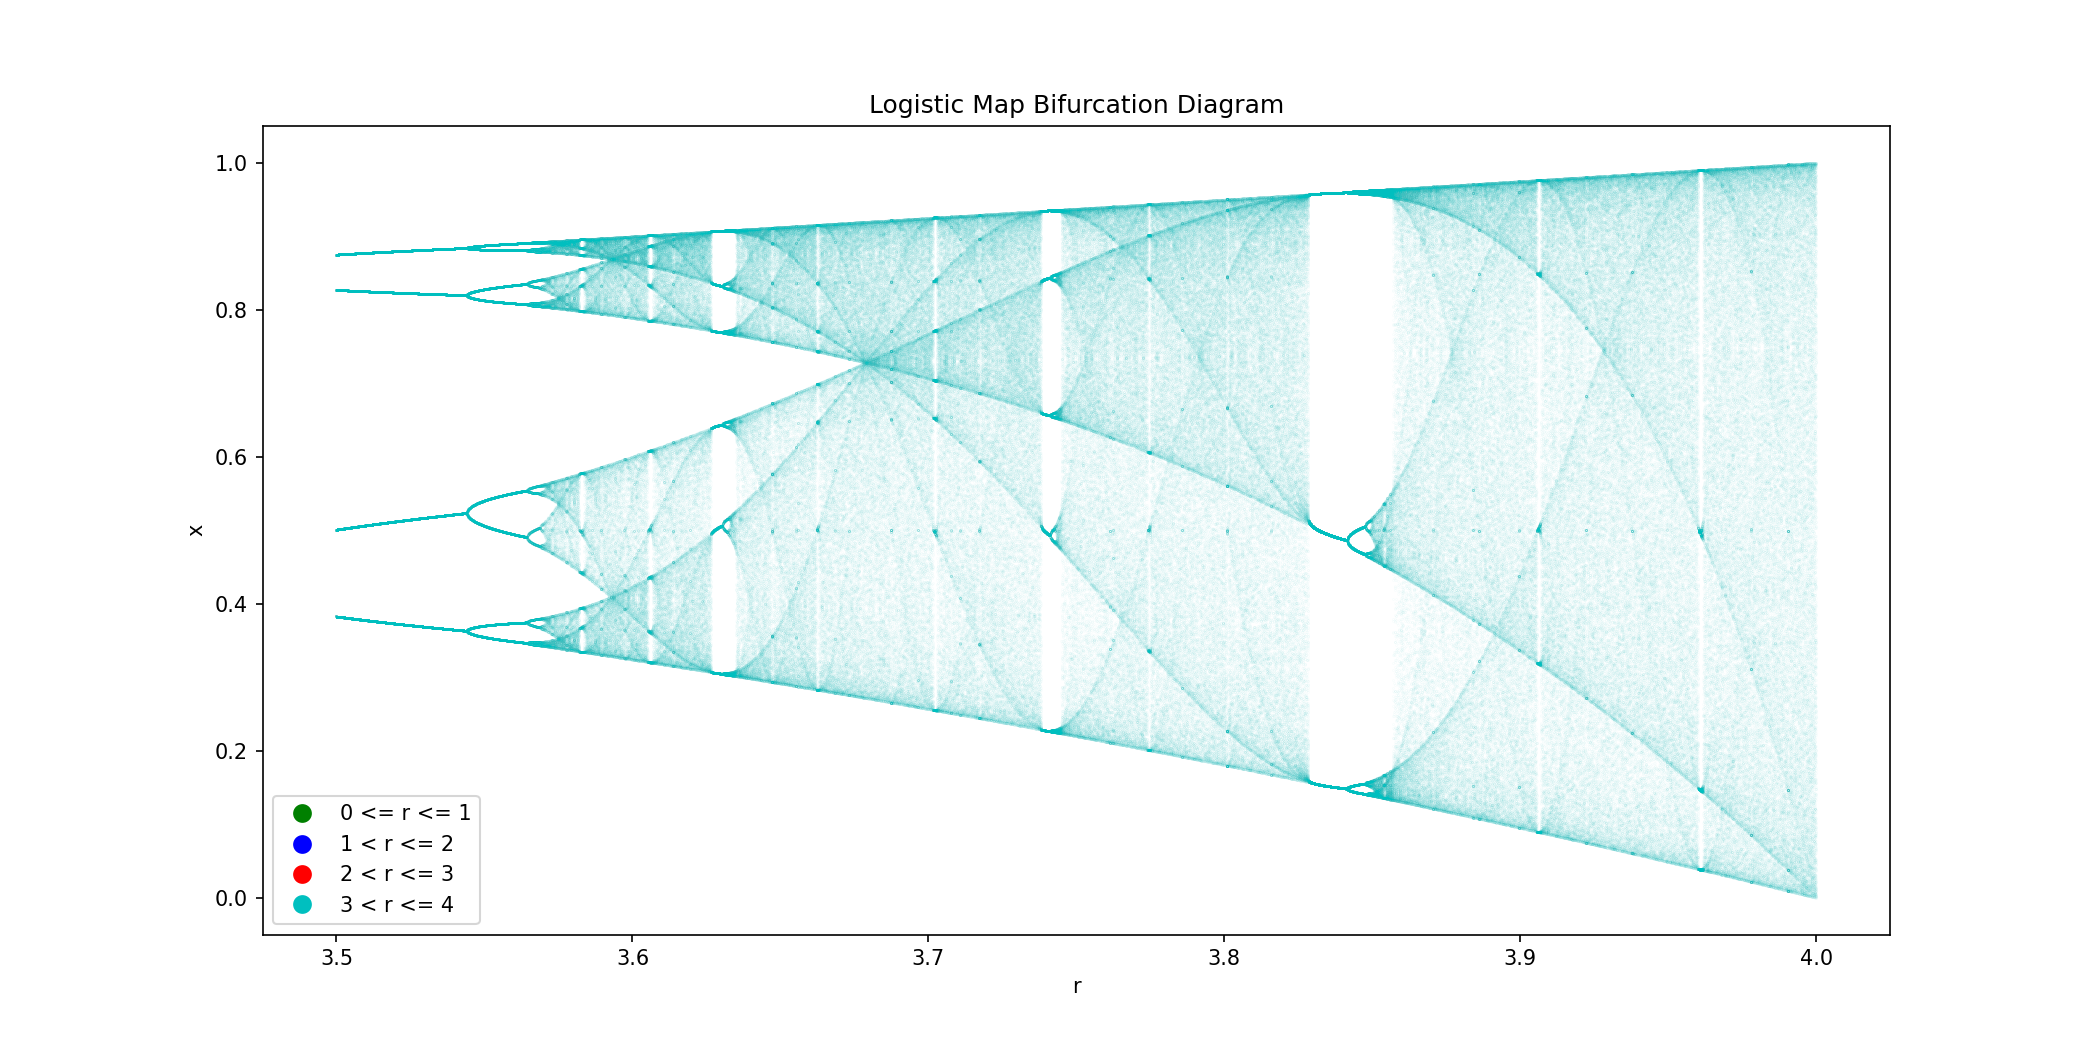
\includegraphics[width=0.75\textwidth]{images/logistic_map_close.png}
    \caption{Logistic map \(r \in [3.5,4]\)}
    \label{r34}
\end{figure}

Finally, in Figure \ref{r04} we can observe the whole diagram for \(r \in [0,4]\). We can notice the stable fixed point at x = 0 when \(0 \le r \le 1\). For \(1 < r \le 3\) we can observe the first period-doubling bifurcation. For \(r > 3\) this orbit continues to split in more period-doubling bifurcations until reaching the critical value we commented before, i.e. \(r \approx 3.57\), when the chaotic behaviour starts, making the system unpredictable and very sensitive to initial conditions.
\begin{figure}[H]
    \centering
    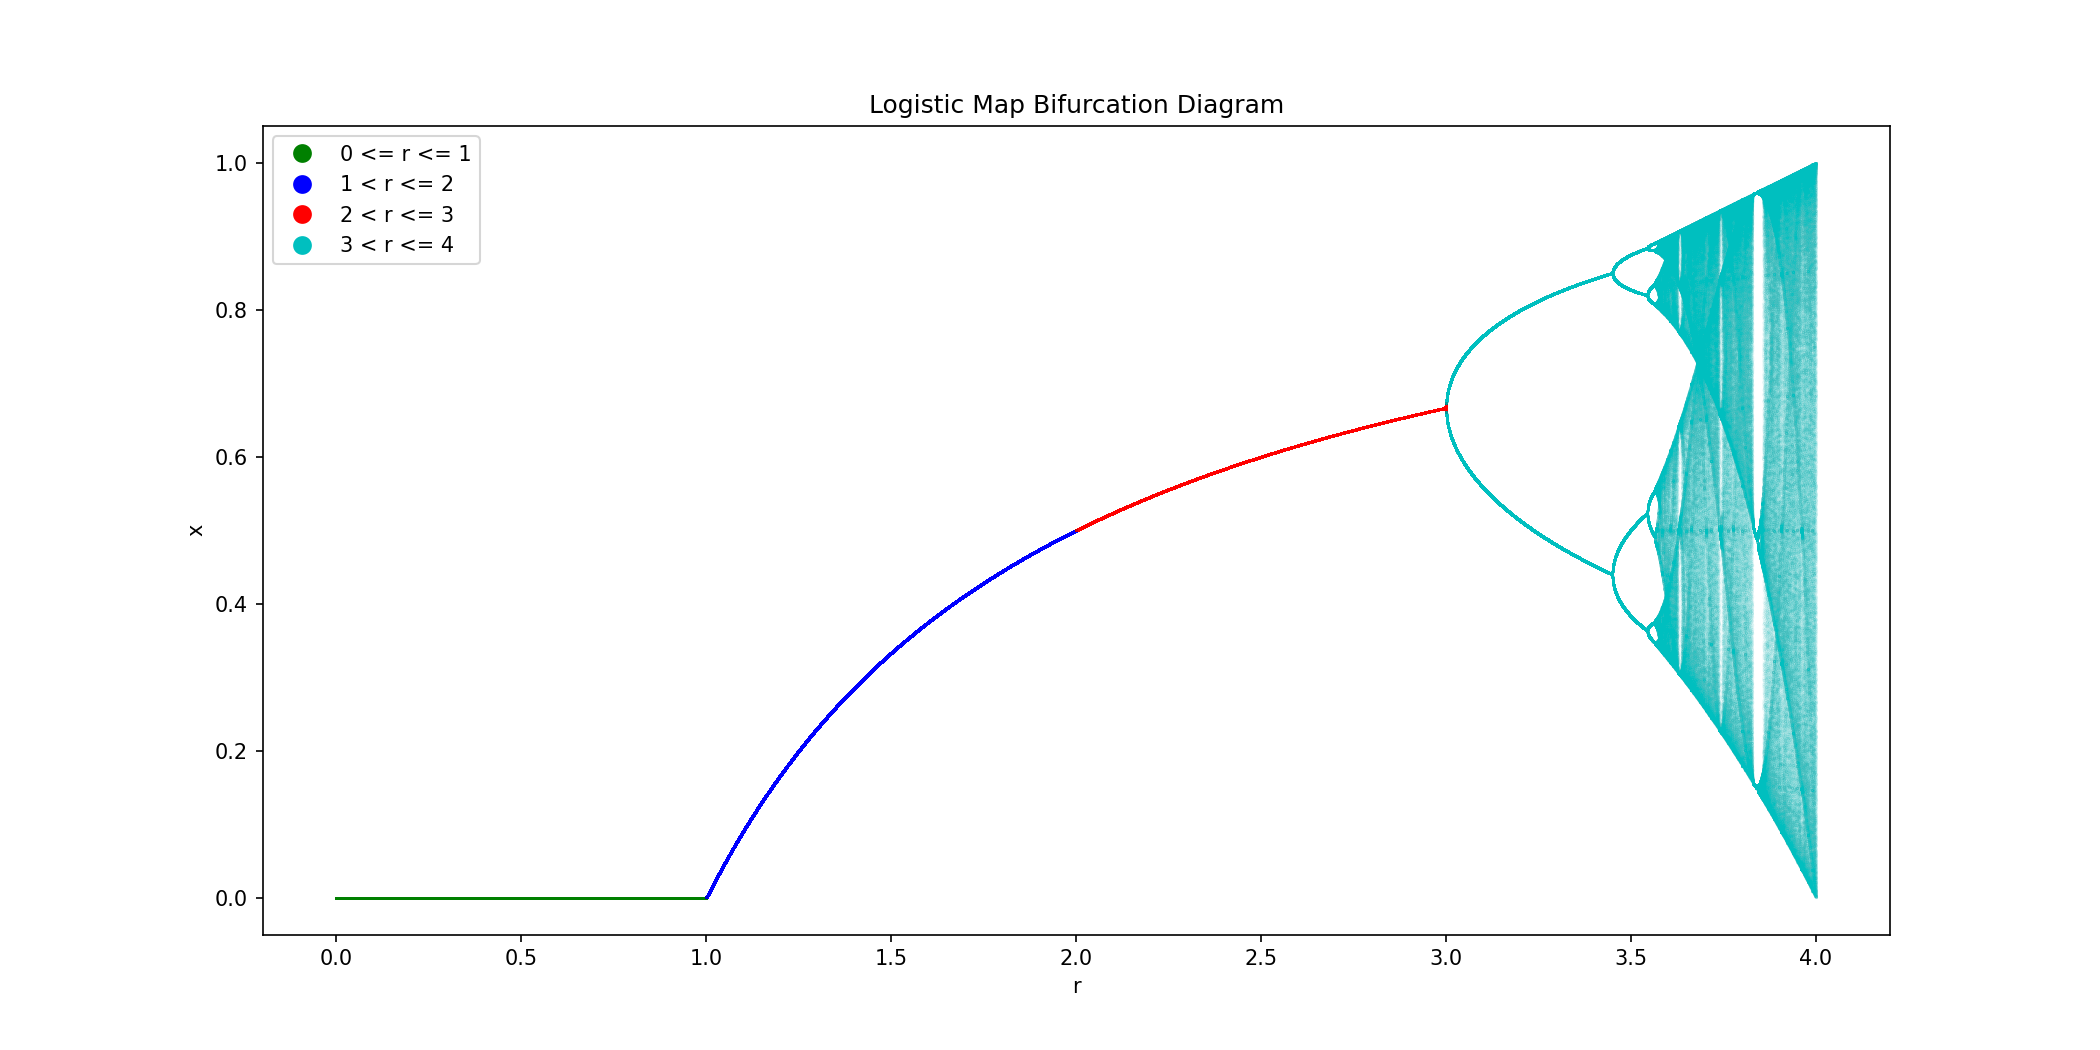
\includegraphics[width=0.75\textwidth]{images/logistic_map_0_4.png}
    \caption{Logistic map \(r \in [0,4]\)}
    \label{r04}
\end{figure}

\paragraph{Lorenz attractor} Now, we will study a system in three-dimensional space that exhibits chaotic behaviour, the Lorenz system.
This system is given by the following equations \cite{lorenz1963deterministic}:
\begin{align*}
\frac{dx}{dt} &= \sigma (y - x) \\
\frac{dy}{dt} &= x (\rho - z) - y \\
\frac{dz}{dt} &= xy - \beta z
\end{align*}

To test the operation of the system, we will start by testing with some initial conditions \(x_0 = (10,10,10)\) and the parameter values \(\sigma = 10, \beta = 8/3, \rho = 28\) for a time \(T_{end} = 1000\). In Figure \ref{lorenzinitial} we can observe the trajectory generated by the system. The trajectory seems to oscillate between two hidden chaotic attractors, as well as a periodic attractor in point \(x = 0\), where the trajectory always passes. The system appears to produce a chaotic trajectory for the given parameters, but we will test this checking its sensitivity to initial conditions.

\begin{figure}[H]
\centering
\subfigure[3D plot]{
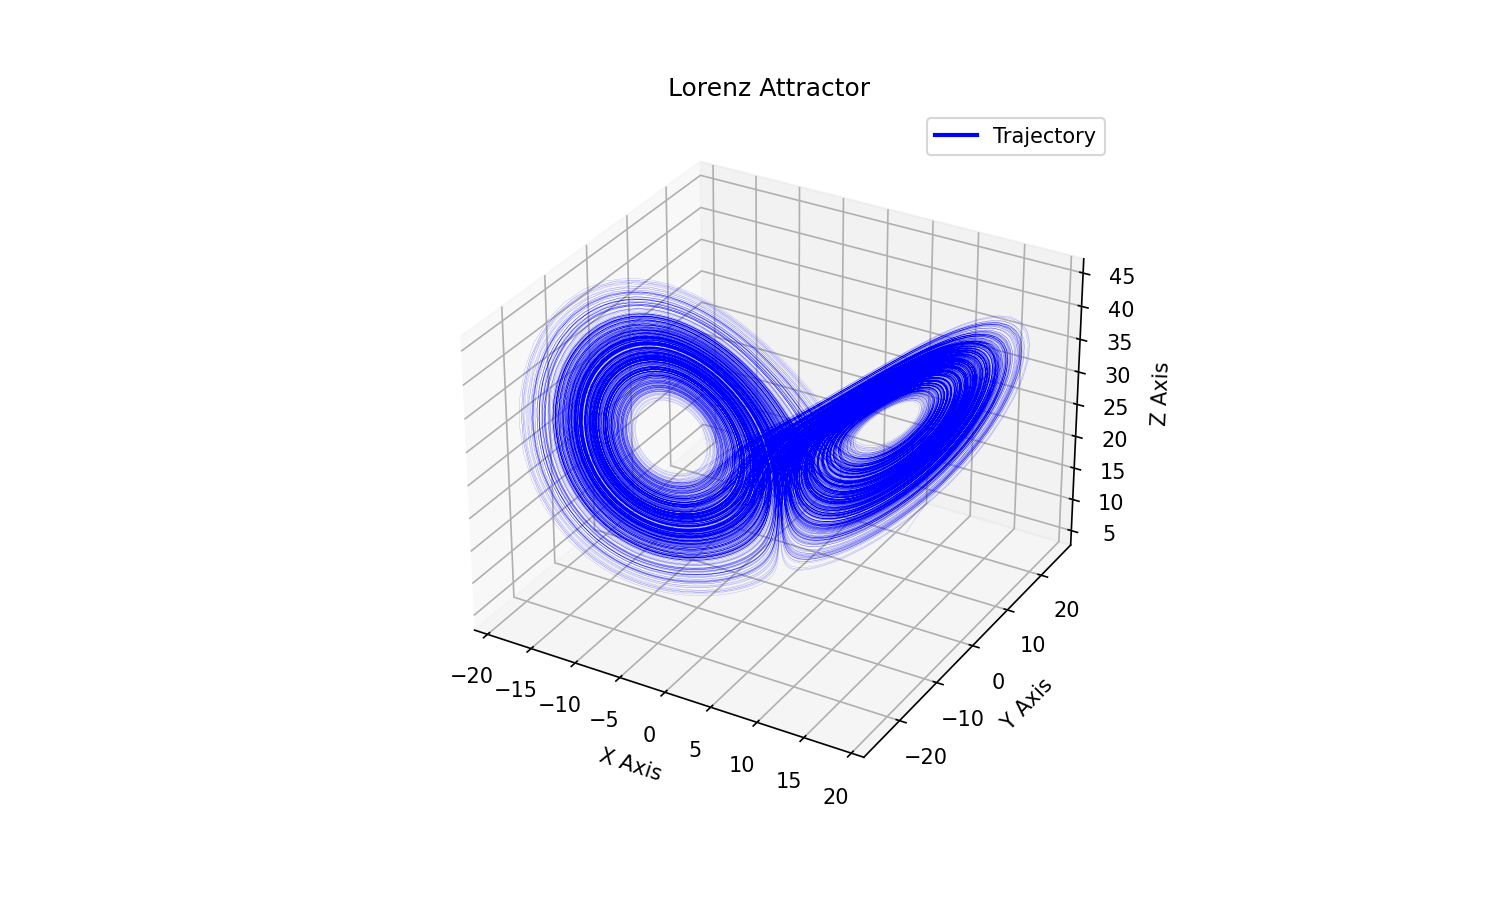
\includegraphics[width=1\textwidth]{images/trajectory_lorentz.png}}
\subfigure[XZ plane plot]{
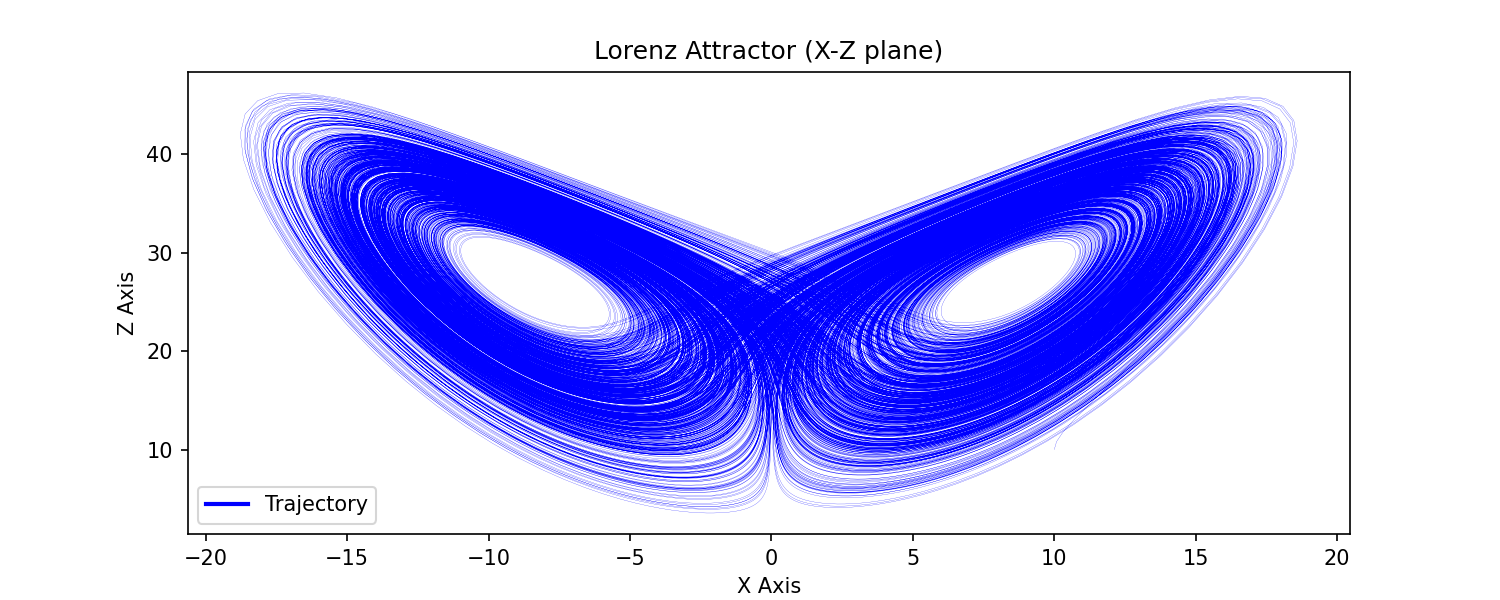
\includegraphics[width=0.75\textwidth]{images/trajectory_lorentz_xz.png}}
\caption{Plots for \(\sigma = 10, \beta = 8/3, \rho = 28\)}
\label{lorenzinitial}
\end{figure}

Therefore, now we will slightly perturb the initial conditions \(x_0\) to \(x_0 = (10 + 10^{-8}, 10, 10)\). Now, we can check the difference between the trajectory with the original initial conditions and the perturbed one.
\begin{figure}[H]
\centering
\subfigure[3D plot]{
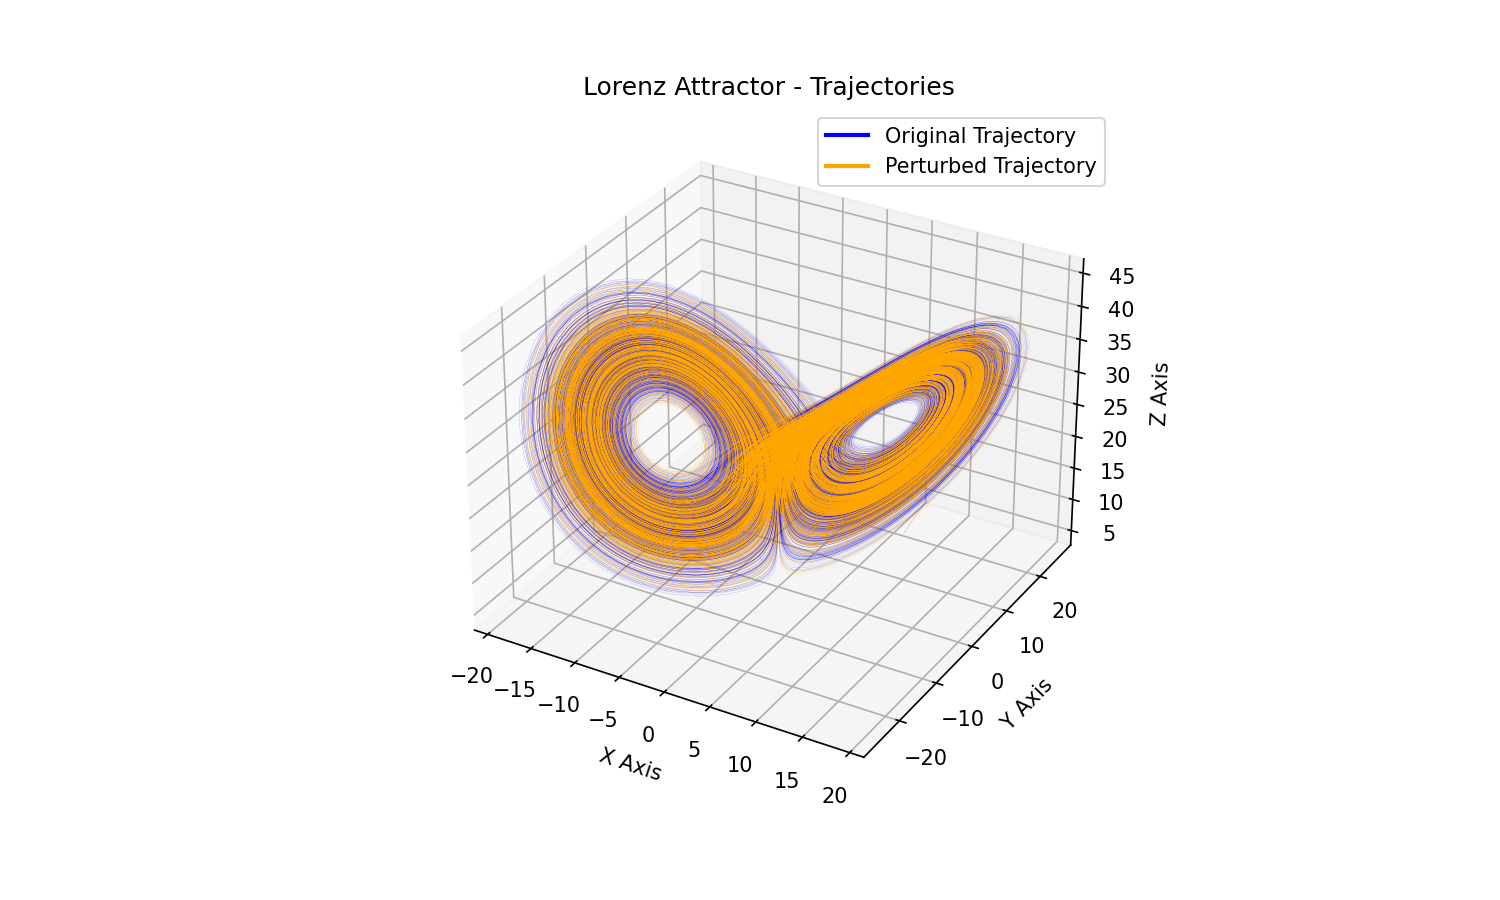
\includegraphics[width=0.75\textwidth]{images/trajectory_lorentz_mul.png}}
\subfigure[XZ plane plot]{
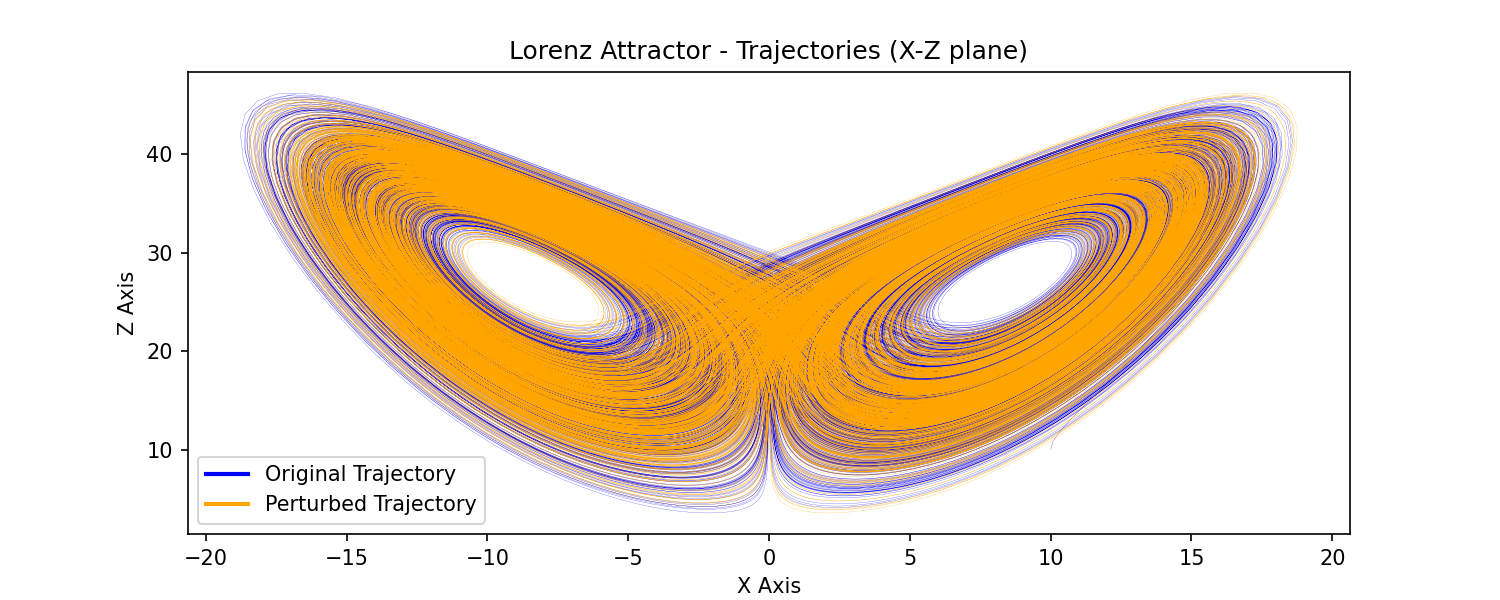
\includegraphics[width=0.75\textwidth]{images/trajectory_lorentz_mul_xz.png}}
\subfigure[Euclidean distance between both trajectories]{
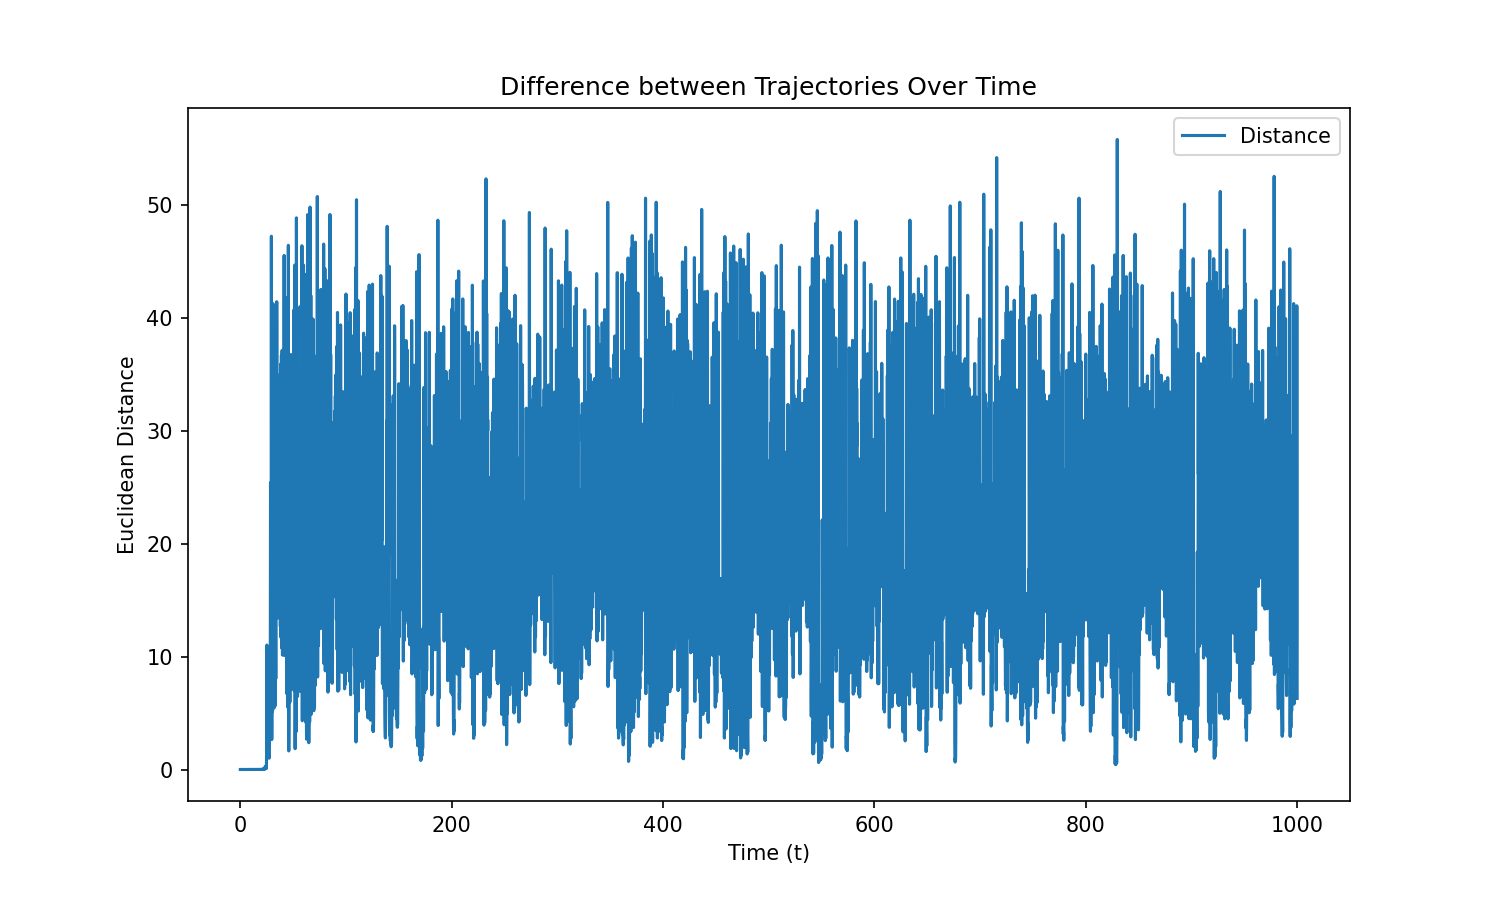
\includegraphics[width=0.5\textwidth]{images/distance_trajectories_1000.png}}
\caption{Comparison between the original and the perturbed trajectories}
\label{lorenzcomparison}
\end{figure}

In Figure \ref{lorenzcomparison}a and \ref{lorenzcomparison}b we can observe that the overall structure of the trajectory is preserved by changing the initial conditions. However, analyzing Figure \ref{lorenzcomparison}c we can check how the Euclidean distance between both trajectories explodes when reaching a certain value. Thus, we can verify that the behaviour of the system is chaotic, since varying the initial conditions by a minimum perturbation results in a trajectory that is very far from the original one. Although they keep the same structure, both trajectories are not the same. 

It is also interesting to note that the distance has peaks but also troughs, which seem to be random, given the chaotic behaviour of the system. However, we also hypothesise that when the distance between the trajectories goes down it is because they are passing through the attractor located at \(x = 0\), where all trajectories end up passing each time.

In order to analyze better when the distance between the trajectories starts to grow, we have run the system only for \(T_{end} = 30\). Now, in Figure \ref{dist30} we can observe how both trajectories are equal until approximately \(t = 23\) where we can note a small perturbation where the distance is greater than 0; however the crucial time is at \(t = 25\) when there is a sudden difference. After that, the distance between them explodes reaching a difference greater than 40 between both trajectories, exhibiting how the chaotic behaviour emerges exponentially fast.

\begin{figure}[H]
    \centering
    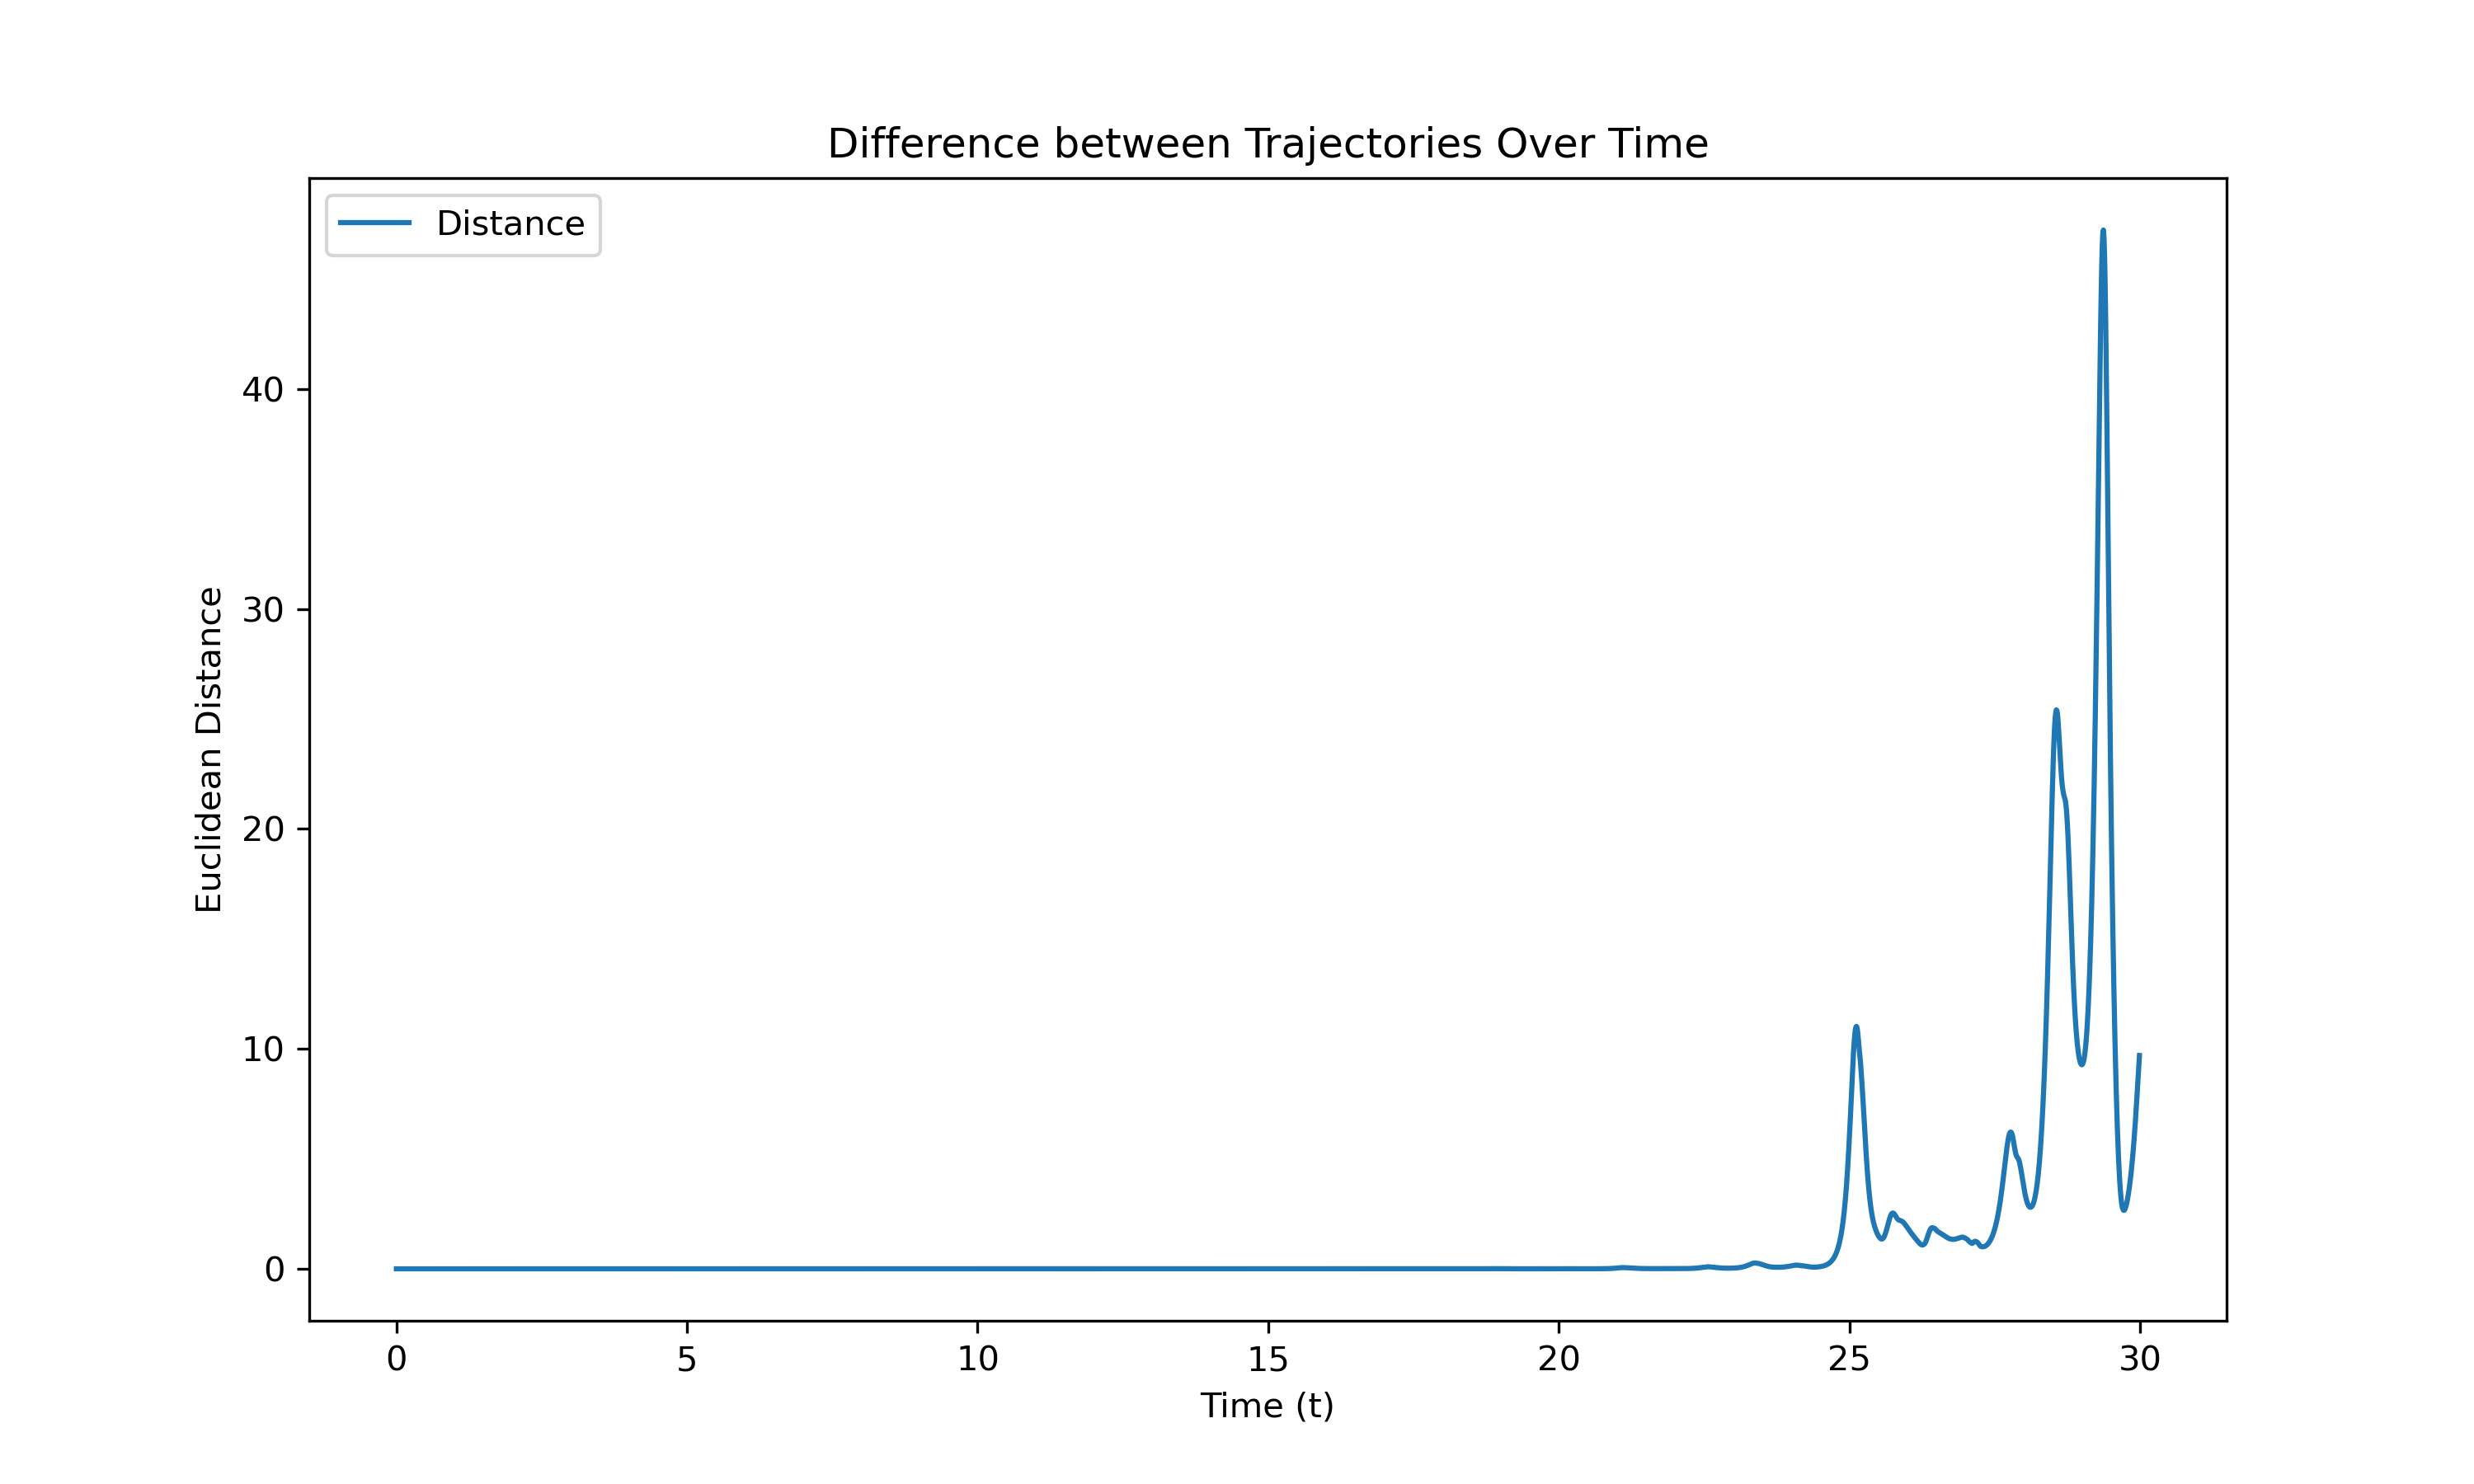
\includegraphics[width=0.75\textwidth]{images/distance_trajectories_30.png}
    \caption{Distance for \(T_{end} = 30\)}
    \label{dist30}
\end{figure}

Now, given the same sets of initial conditions as before, we will check how changing the parameter \(\rho\) changes the system's behaviour. We first try \(\rho = 0.5\), that can be observed in Figure \ref{lorenzrho05}. Now, it is clear that the system is not chaotic anymore. Both trajectories converge to the same point (0,0,0), being their euclidean distance 0 for almost all the time, and its farthest point being at t = 0, where its distance is \(10^{-8}\), the initial perturbation value added. Thus, the system is not chaotic with this parameter configuration, due to it not being sensitive to initial conditions and then being predictable.

\begin{figure}[H]
\centering
\subfigure[3D plot]{
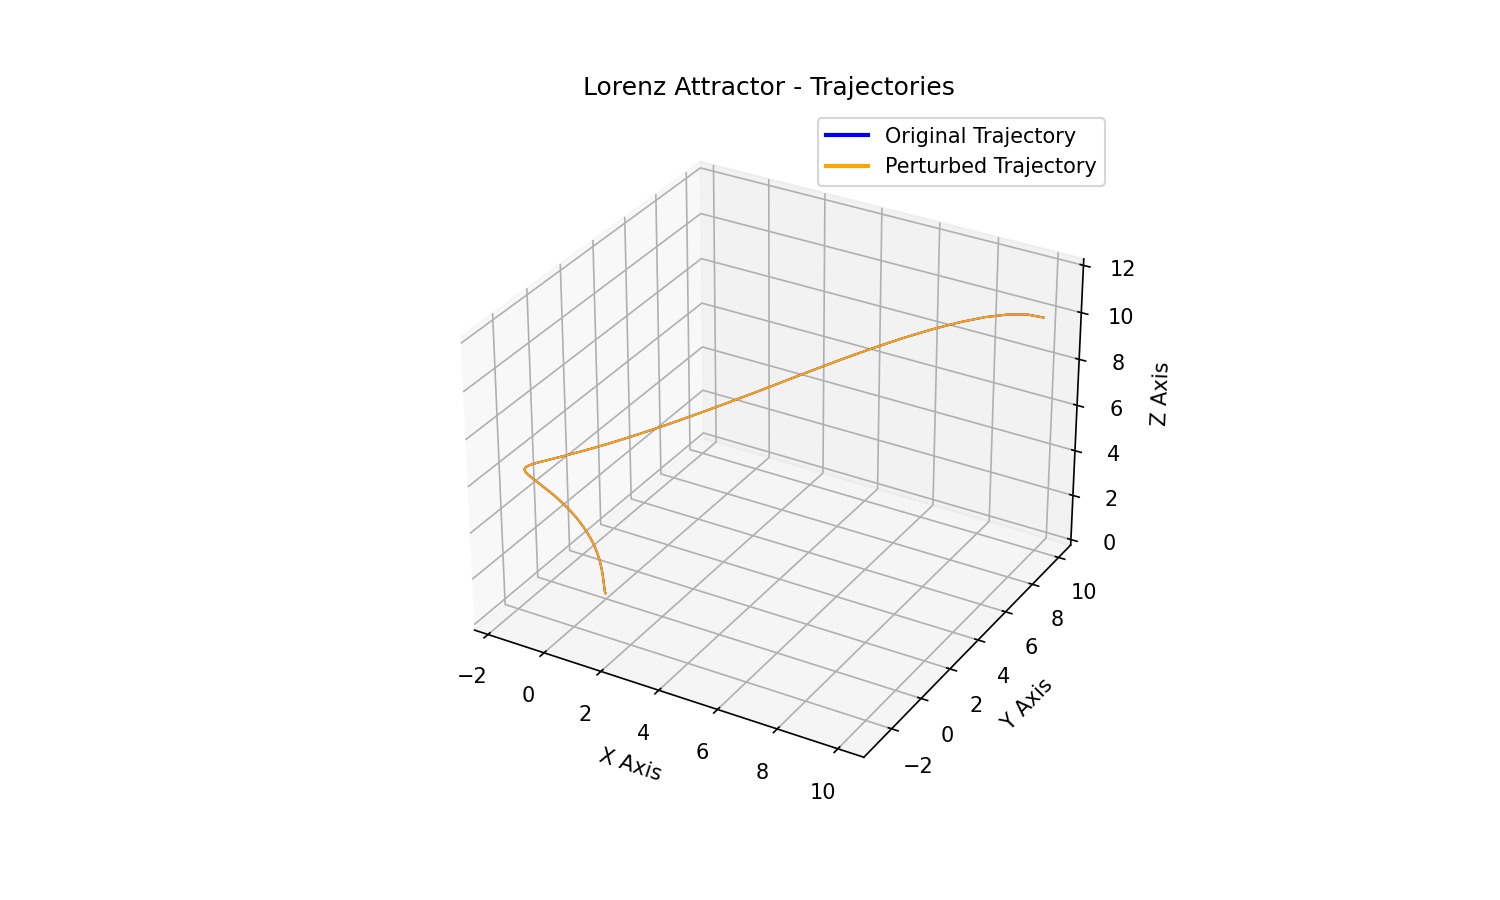
\includegraphics[width=0.75\textwidth]{images/trajectory_lorentz_mul_rho05.png}}
\subfigure[XZ plane plot]{
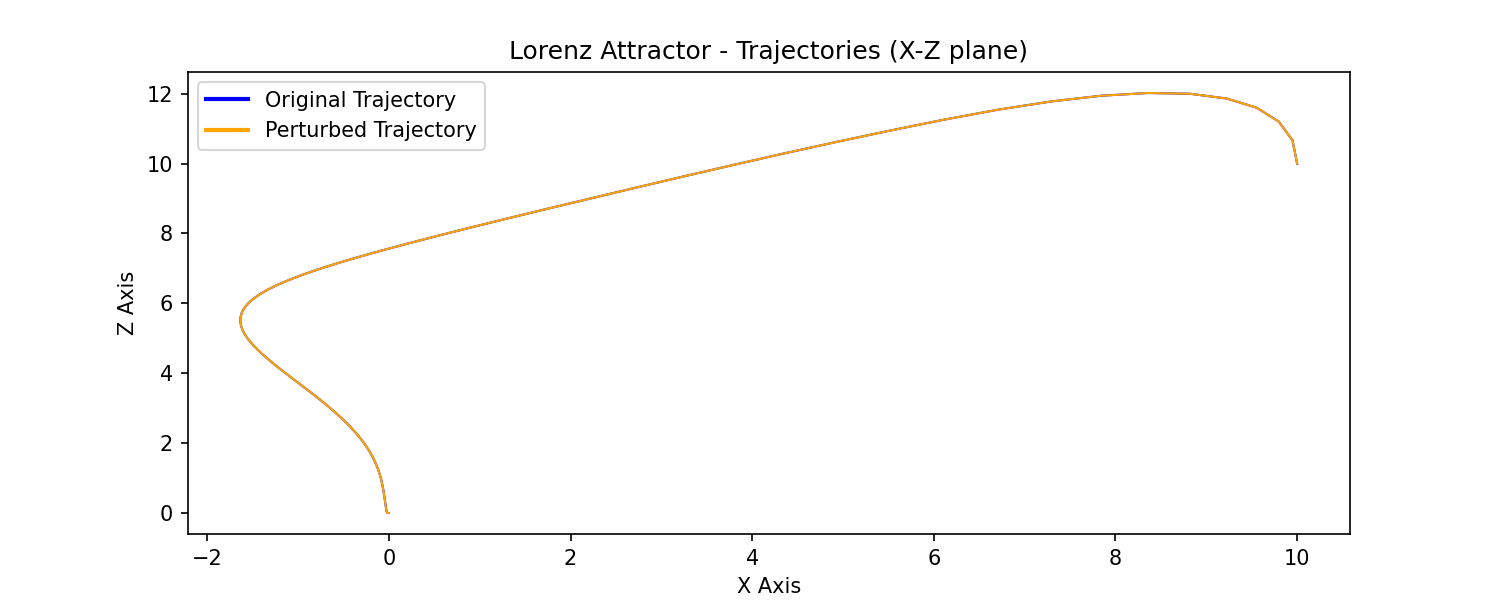
\includegraphics[width=0.75\textwidth]{images/trajectory_lorentz_mul_xz_rho05.png}}
\subfigure[Euclidean distance between both trajectories]{
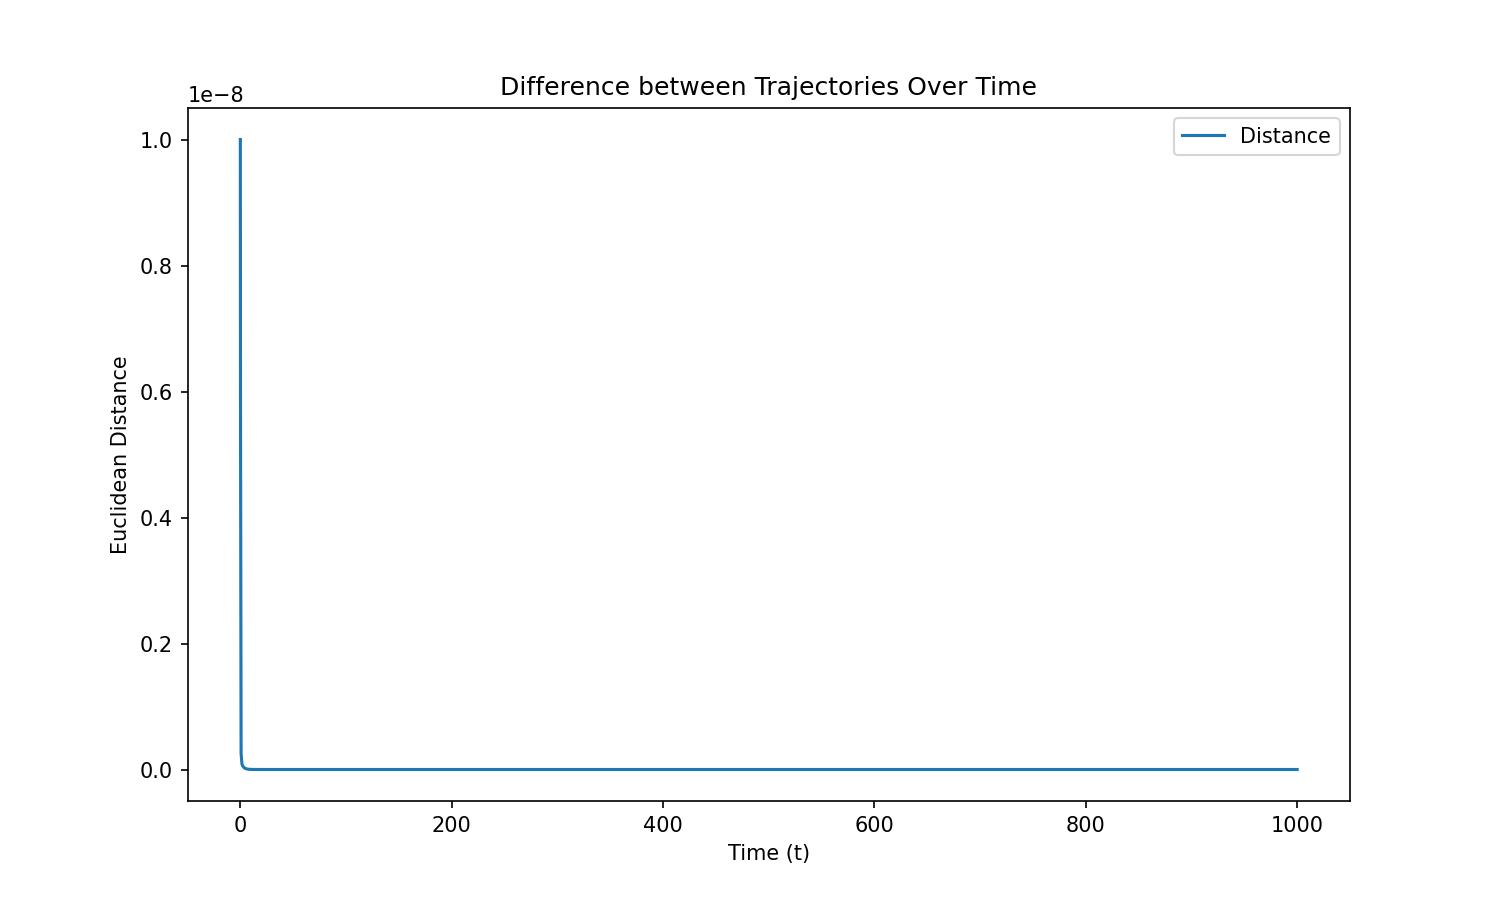
\includegraphics[width=0.5\textwidth]{images/distance_trajectories_rho05.png}}
\caption{Comparison for \(\rho = 0.5\)}
\label{lorenzrho05}
\end{figure}

Also, we know that the Lorenz system is chaotic for \((\sigma = 10, \beta = 8/3, \rho = 28\) and nearby values \cite{hirsch2012differential}. Therefore, when trying other values for \(\rho\) like \(\rho = 5\) it is not surprising to see the same non-chaotic behaviour as before. We also increased the perturbed \(x_0\) to be \(x_0 = (10+5, 10, 10)\). Again, in Figure \ref{lorenzrho5} we can observe that the system is not chaotic, not being so sensitive to the initial conditions. Also, we can see better how both trajectories are being attracted by an attractor, executing a spiral trajectory. This also can be noted in Figure \ref{lorenzrho5}c, where the distance starts at 5, the perturbation value, and strictly decreases until it is 0.

\begin{figure}[H]
\centering
\subfigure[3D plot]{
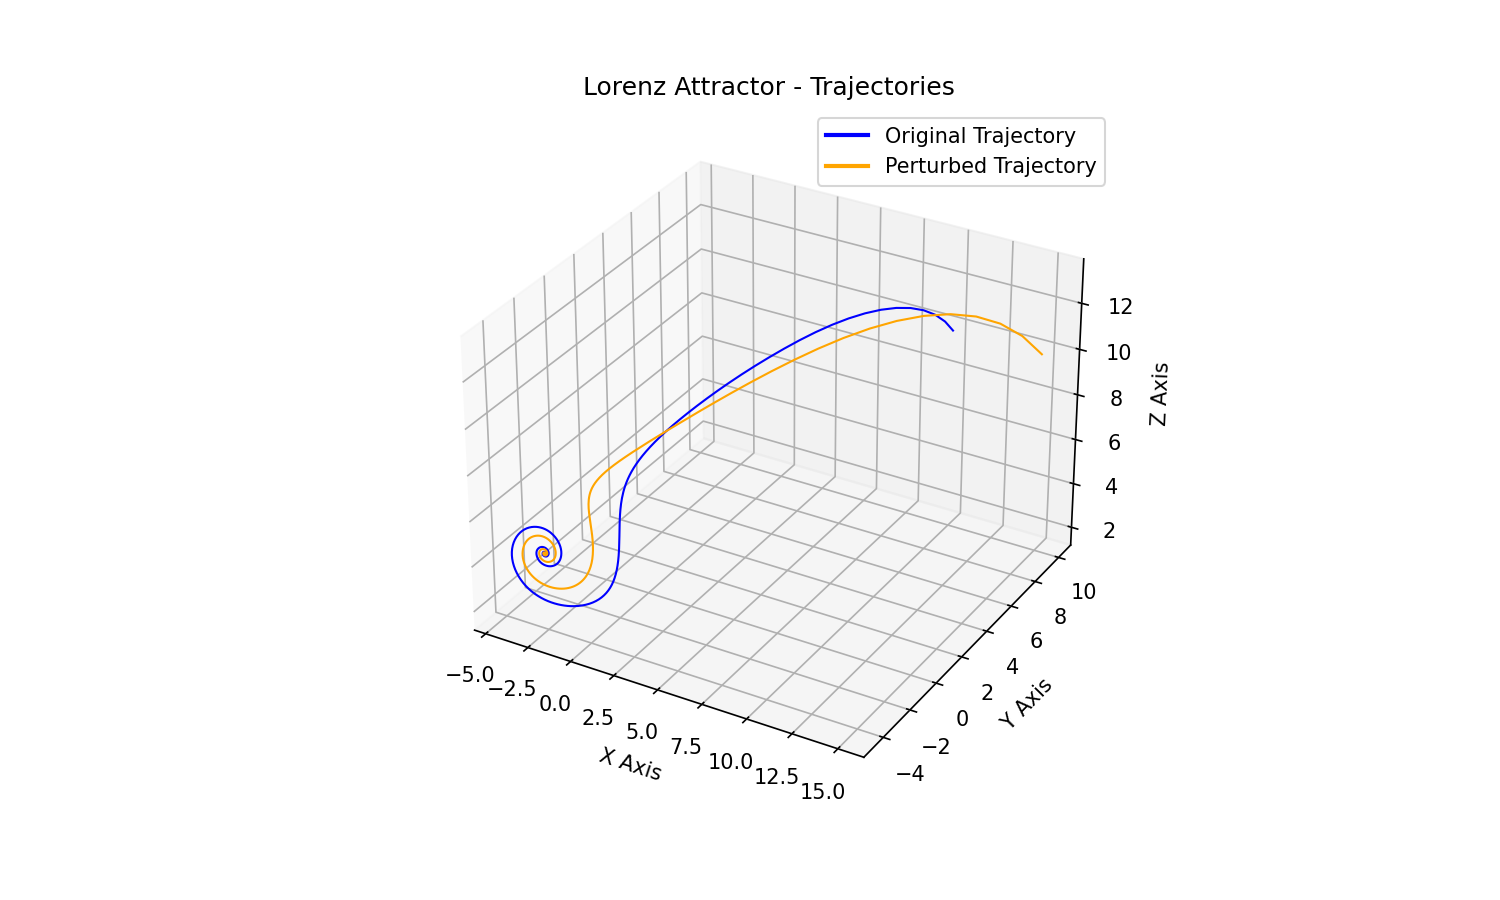
\includegraphics[width=0.75\textwidth]{images/trajectory_lorentz_mul_rho5.png}}
\subfigure[XZ plane plot]{
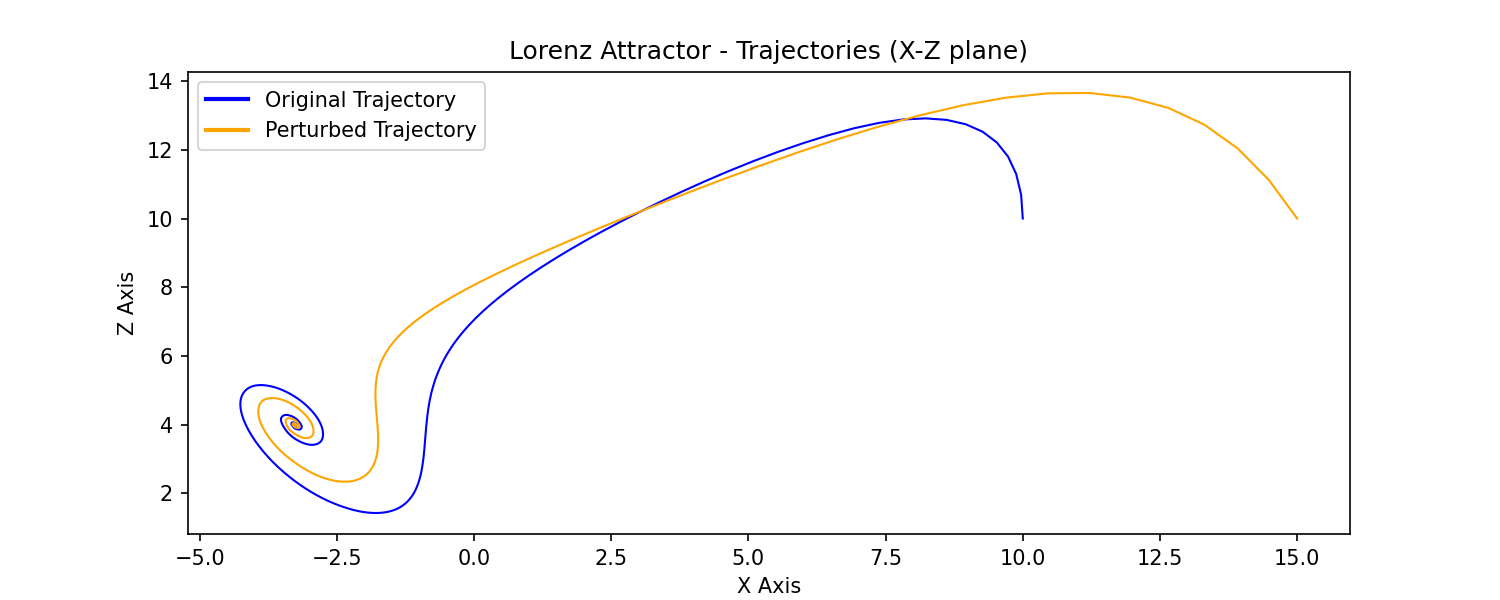
\includegraphics[width=0.75\textwidth]{images/trajectory_lorentz_mul_xz_rho5.png}}
\subfigure[Euclidean distance between both trajectories]{
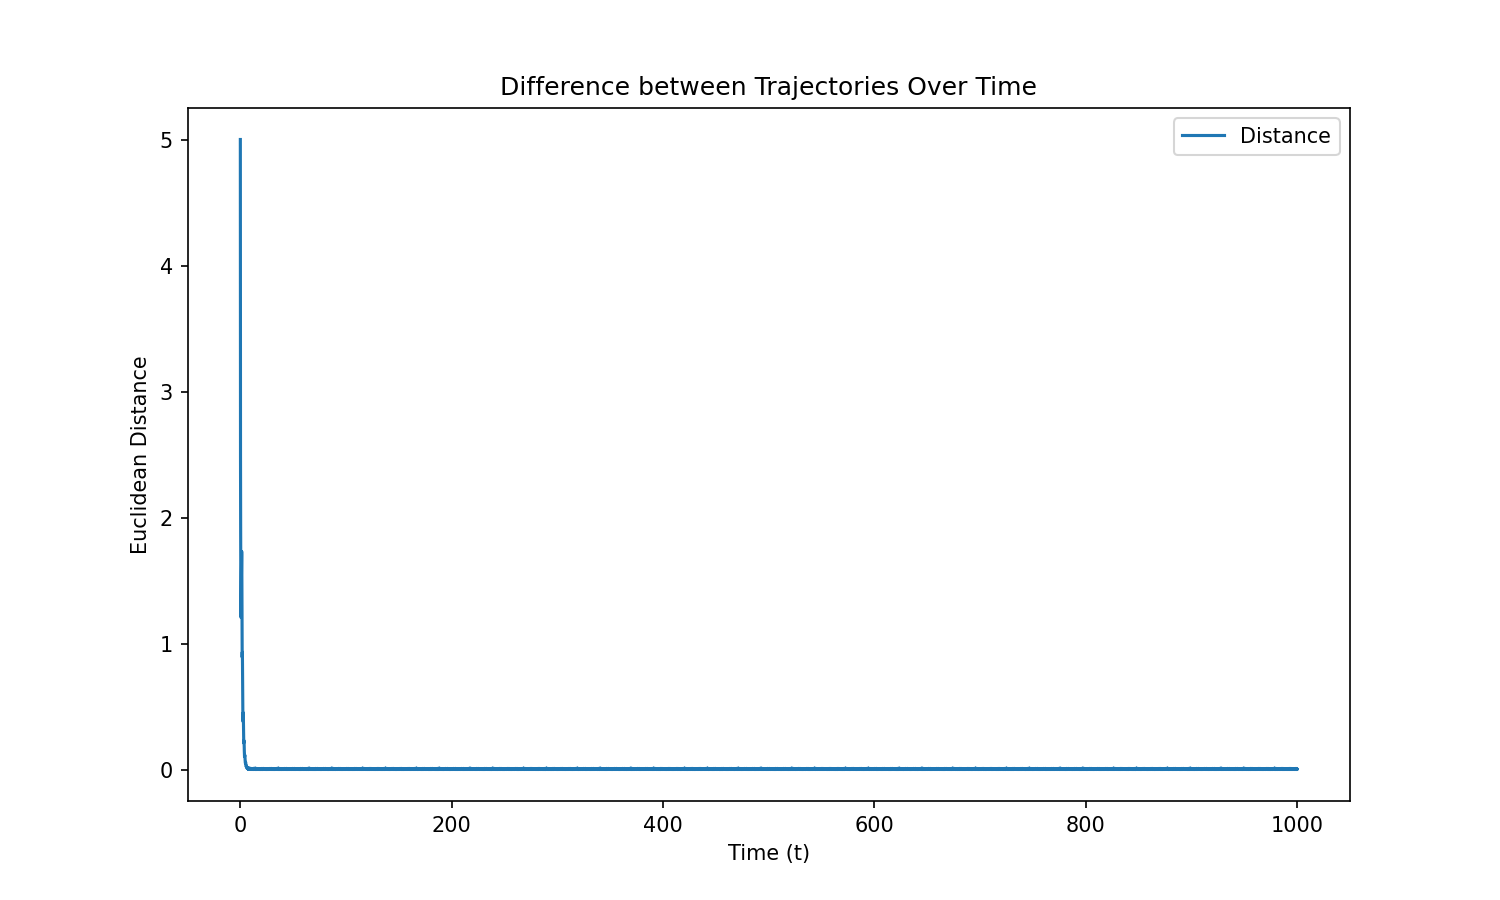
\includegraphics[width=0.5\textwidth]{images/distance_trajectories_rho5.png}}
\caption{Comparison for \(\rho = 5\)}
\label{lorenzrho5}
\end{figure}

Finally, we can answer the question: Is there a bifurcation (or multiple ones) between the value \(\rho = 0.5\) and \(\rho = 28\)? Given the definition of a bifurcation: "The appearance of a topologically nonequivalent phase portrait under variation of parameters is called a bifurcation". Consequently, the question can be resolved by determining whether the systems at these parameter values are topologically equivalent. 

Looking at the corresponding Figures for each \(\rho\) value (Figure \ref{lorenzinitial}, \ref{lorenzrho05}) we can clearly see that there is no homeomorphism that maps the orbit of the system with \(\rho = 0.5\) to the system with \(\rho = 28\). To elucidate, it becomes evident that no function can be found that effectively maps the predictable behavior of the first system to the extreme sensitivity to initial conditions exhibited by the latter system. Each infinitesimal change in the initial conditions of the latter system would necessitate a new mapping for the first one, precluding the identification of a unique map. This reasoning similarly applies to the comparison of systems with \(\rho = 5\) and \(\rho = 28\).
\end{task}